\chapter{DNS Configuration with CoreDNS}

In this Section we are going to setup a Kàthara node to reach DNS server

\section{Lab.conf}
 First step is, we need to add some configurations to the conf file we created in the previous assignment.
 \begin{figure}[H]
\centering
  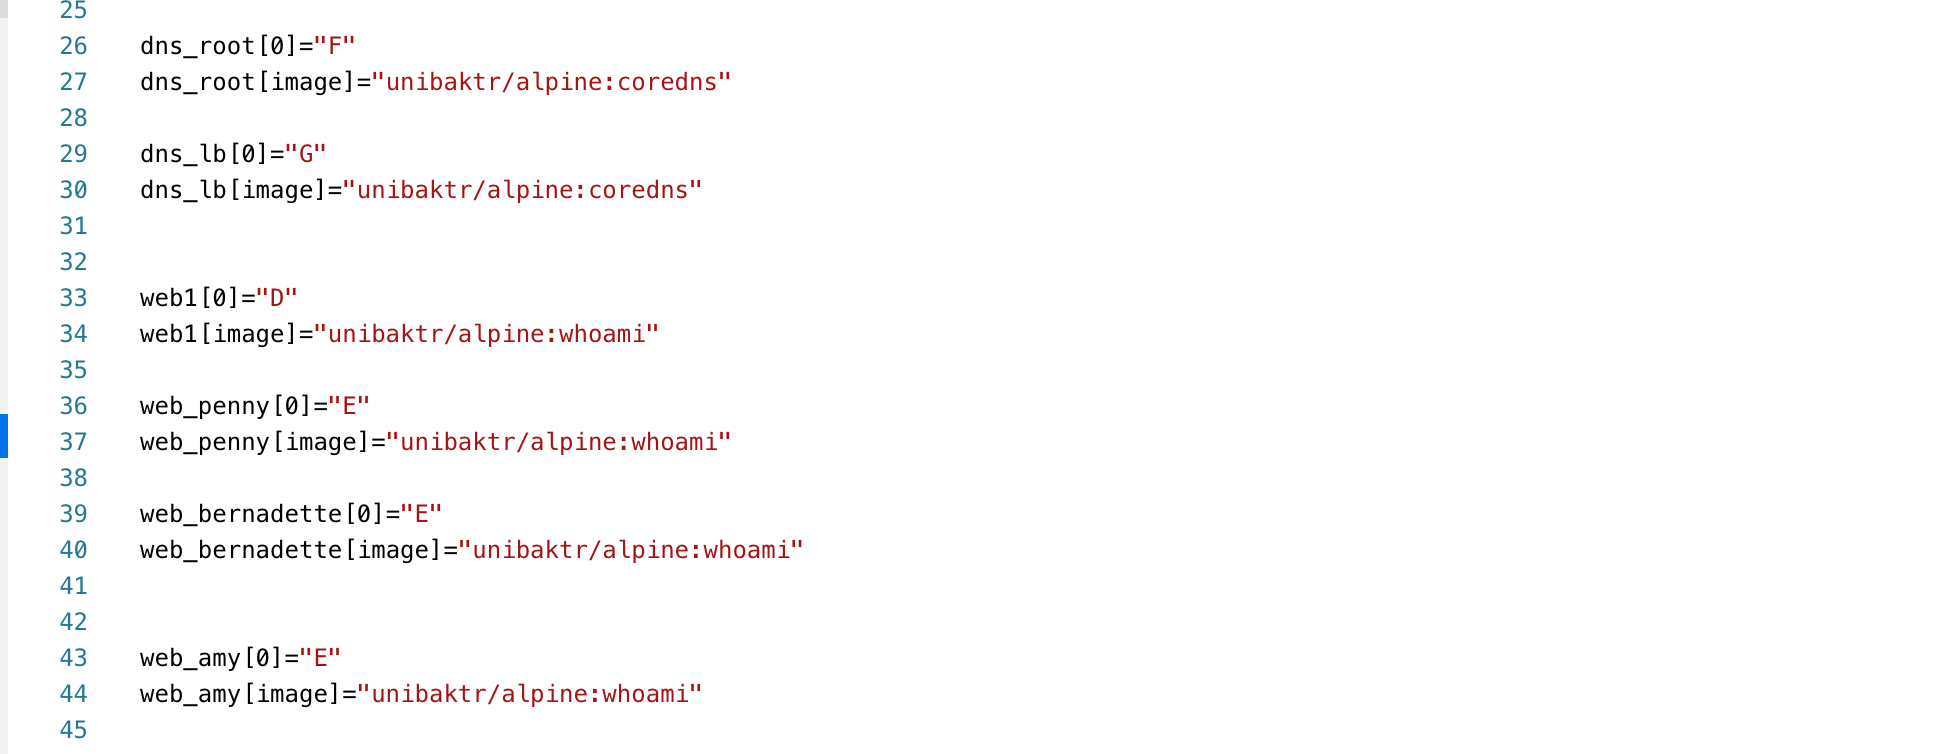
\includegraphics[width=0.9\textwidth]{Images/confAdditions.png}
  \caption{Adding new nodes and configure there images and interfaces in Kàthara lab conf file}
  \label{fig:2.1}
\end{figure}
\section{Startup files}
Second step we need to also configure the startup files for each new node and configure there routes so the whole network would be connected.

 \begin{figure}[H]
\centering
  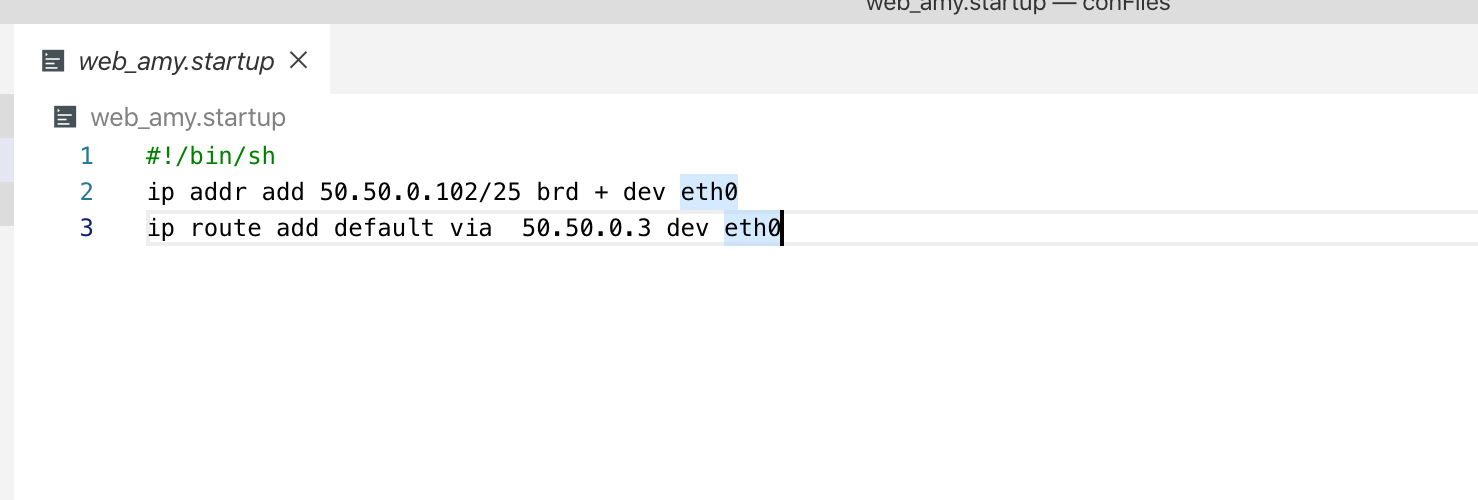
\includegraphics[width=0.9\textwidth]{Images/startupExample.png}
  \caption{Example for new added nodes setup file with configuring it's route}
  \label{fig:2.2}
\end{figure}


\section{Setup a Kàthara node to reach DNS server}
Third, We will setup dns\_root to be an authoritative server for the root domain and de. In order to do that we will need to create a folder with the same name of the node. The folder will contain three main files.
\subsection{Corefile file}
Corfile is used to configure coreDns. When coreDns runs the first thing it will do, look for a file named \textbf{Corefile}. In coreFile we define the Server blocks we will use. In this section we will use two server blocks. The first one is the root \textbf{\.} which is responsible for all zones below the root zone. The second server block we will us is \textbf{de} zone.

 \begin{figure}[H]
\centering
  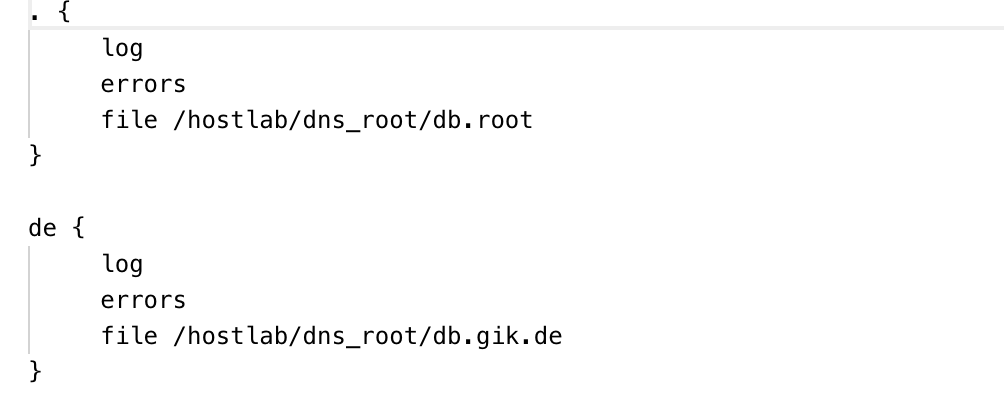
\includegraphics[width=0.9\textwidth]{Images/coreFilednsRoot.png}
  \caption{Corefile for dns\_root node with root and de Server blocks}
  \label{fig:2.3}
\end{figure}
As we can see in the coreFile we are calling two more files \textbf{db.root} and \textbf{db.gik.de}. Now the question what are those files. This files are used to support and define  one or more zone.
\subsection{db.root}
In this file will define the root server and how the protocol will be as in \ref{fig:2.4}
you will see that you define the TTl (Time to live) which is how much time packets will stay in that network and then you fined that you define some attributes for the server like expire time , cache time .. etc. Then you will make the root server look to the ip of de as shown.

 \begin{figure}[H]
\centering
  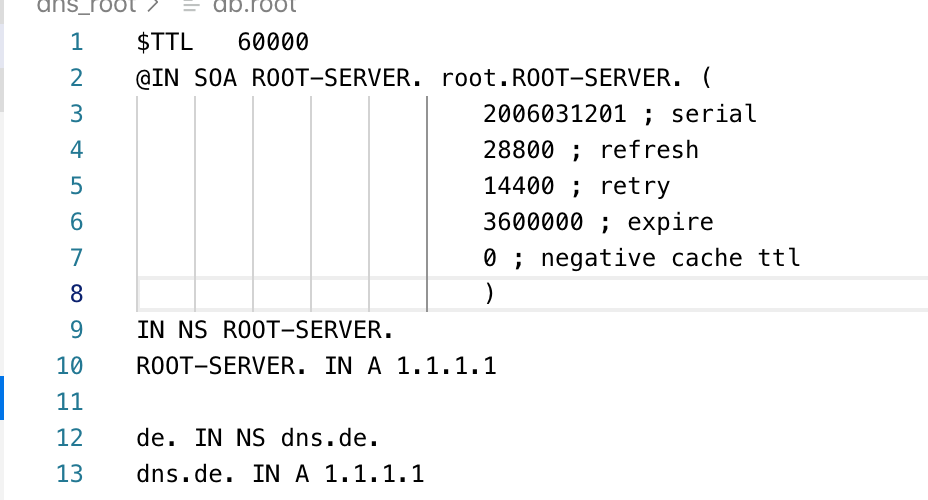
\includegraphics[width=0.9\textwidth]{Images/dpRoot.png}
  \caption{db.root file}
  \label{fig:2.4}
\end{figure}
\subsection{db.gik.de}

In this file will define dns.de  and how the protocol will be as in \ref{fig:2.5}. Notice it is same as \ref{fig:2.4} but instead you will make dns.de server look to gik and make it point to the ip of web1.

 \begin{figure}[H]
\centering
  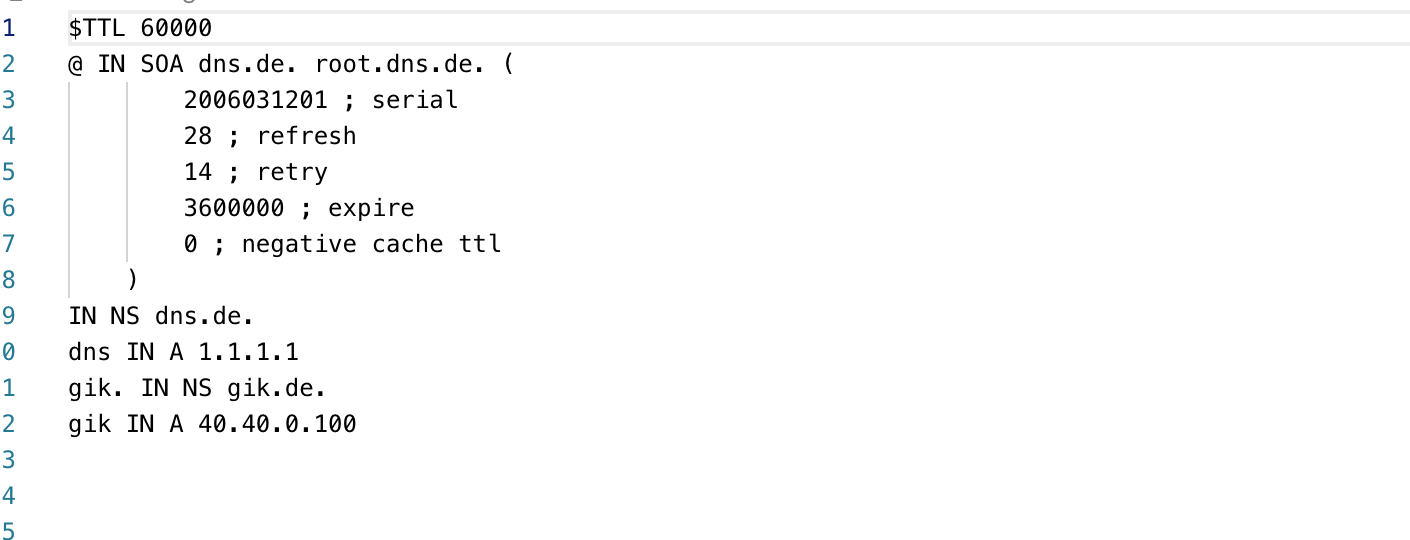
\includegraphics[width=0.9\textwidth]{Images/dpGik.png}
  \caption{db.root file}
  \label{fig:2.5}
\end{figure}

\section{Add name server to pc1 and pc2}
Now we will add nameserver entry to pc1 and pc2 that points to dns\_root and then will test the connectivity using curl from any pc as shown in \ref{fig:2.6} for pc1.
\begin{figure}[H]
\centering
  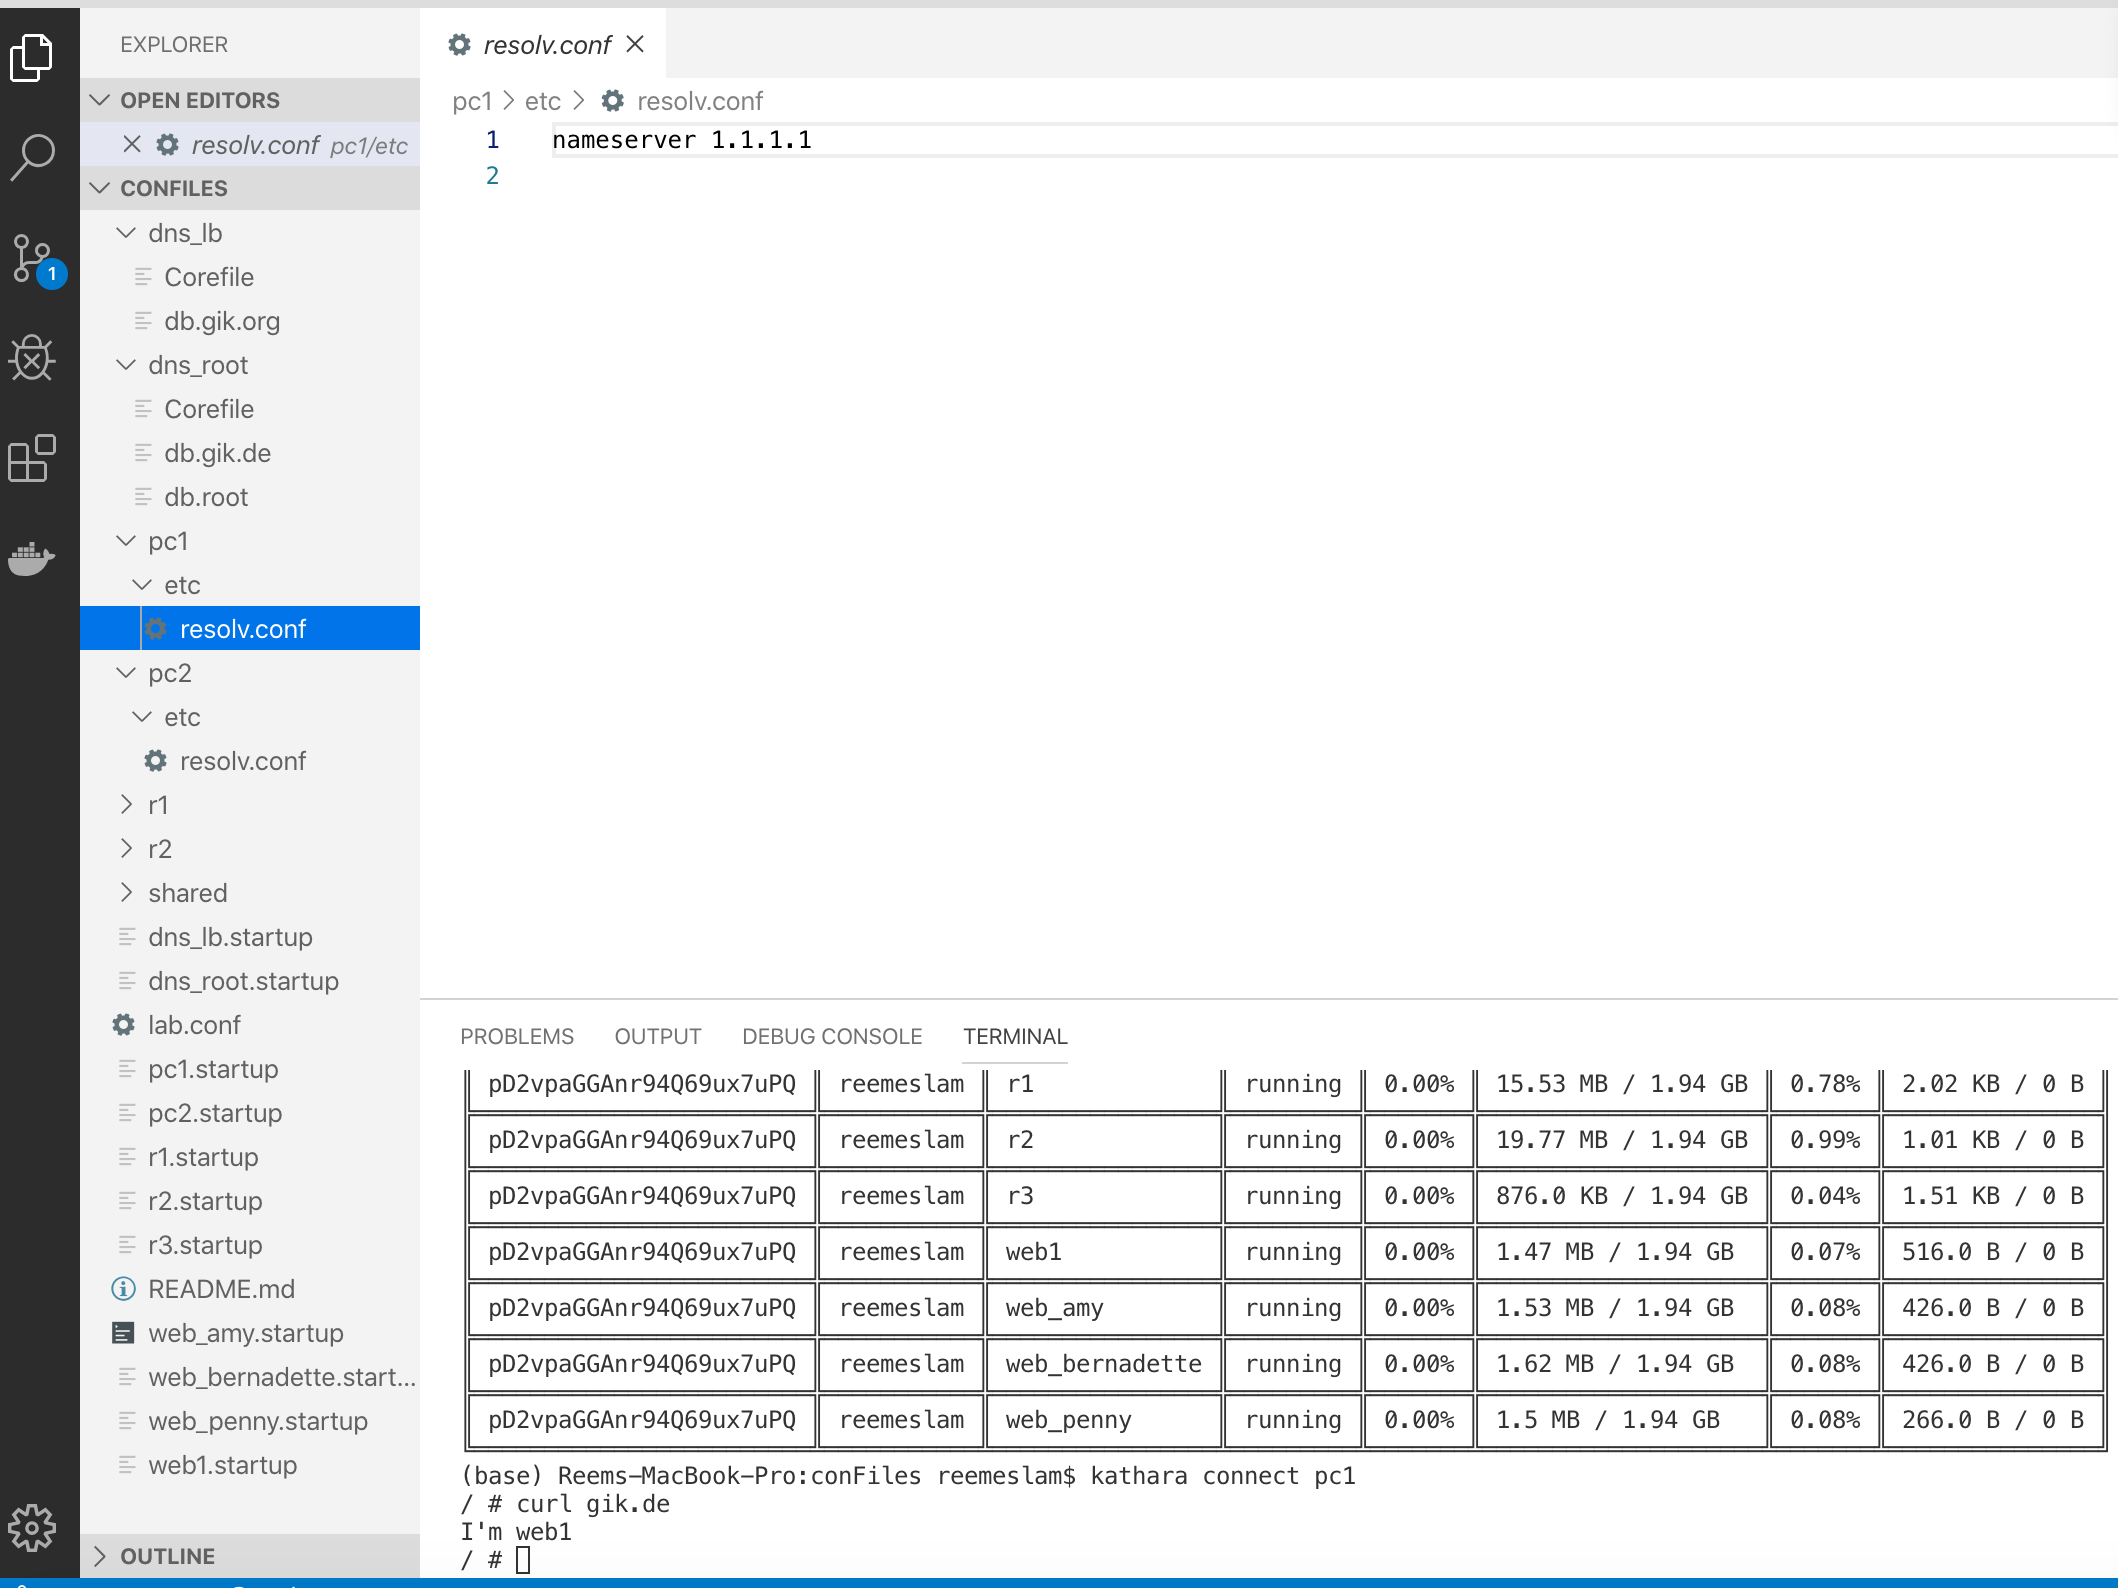
\includegraphics[width=0.9\textwidth]{Images/nameServer.png}
  \caption{Adding nameserver to pc1 and testing that with curl gik.de}
  \label{fig:2.6}
\end{figure}

\section{Capturing the name resolution on CD A  with wireshark}

\begin{figure}[H]
\centering
  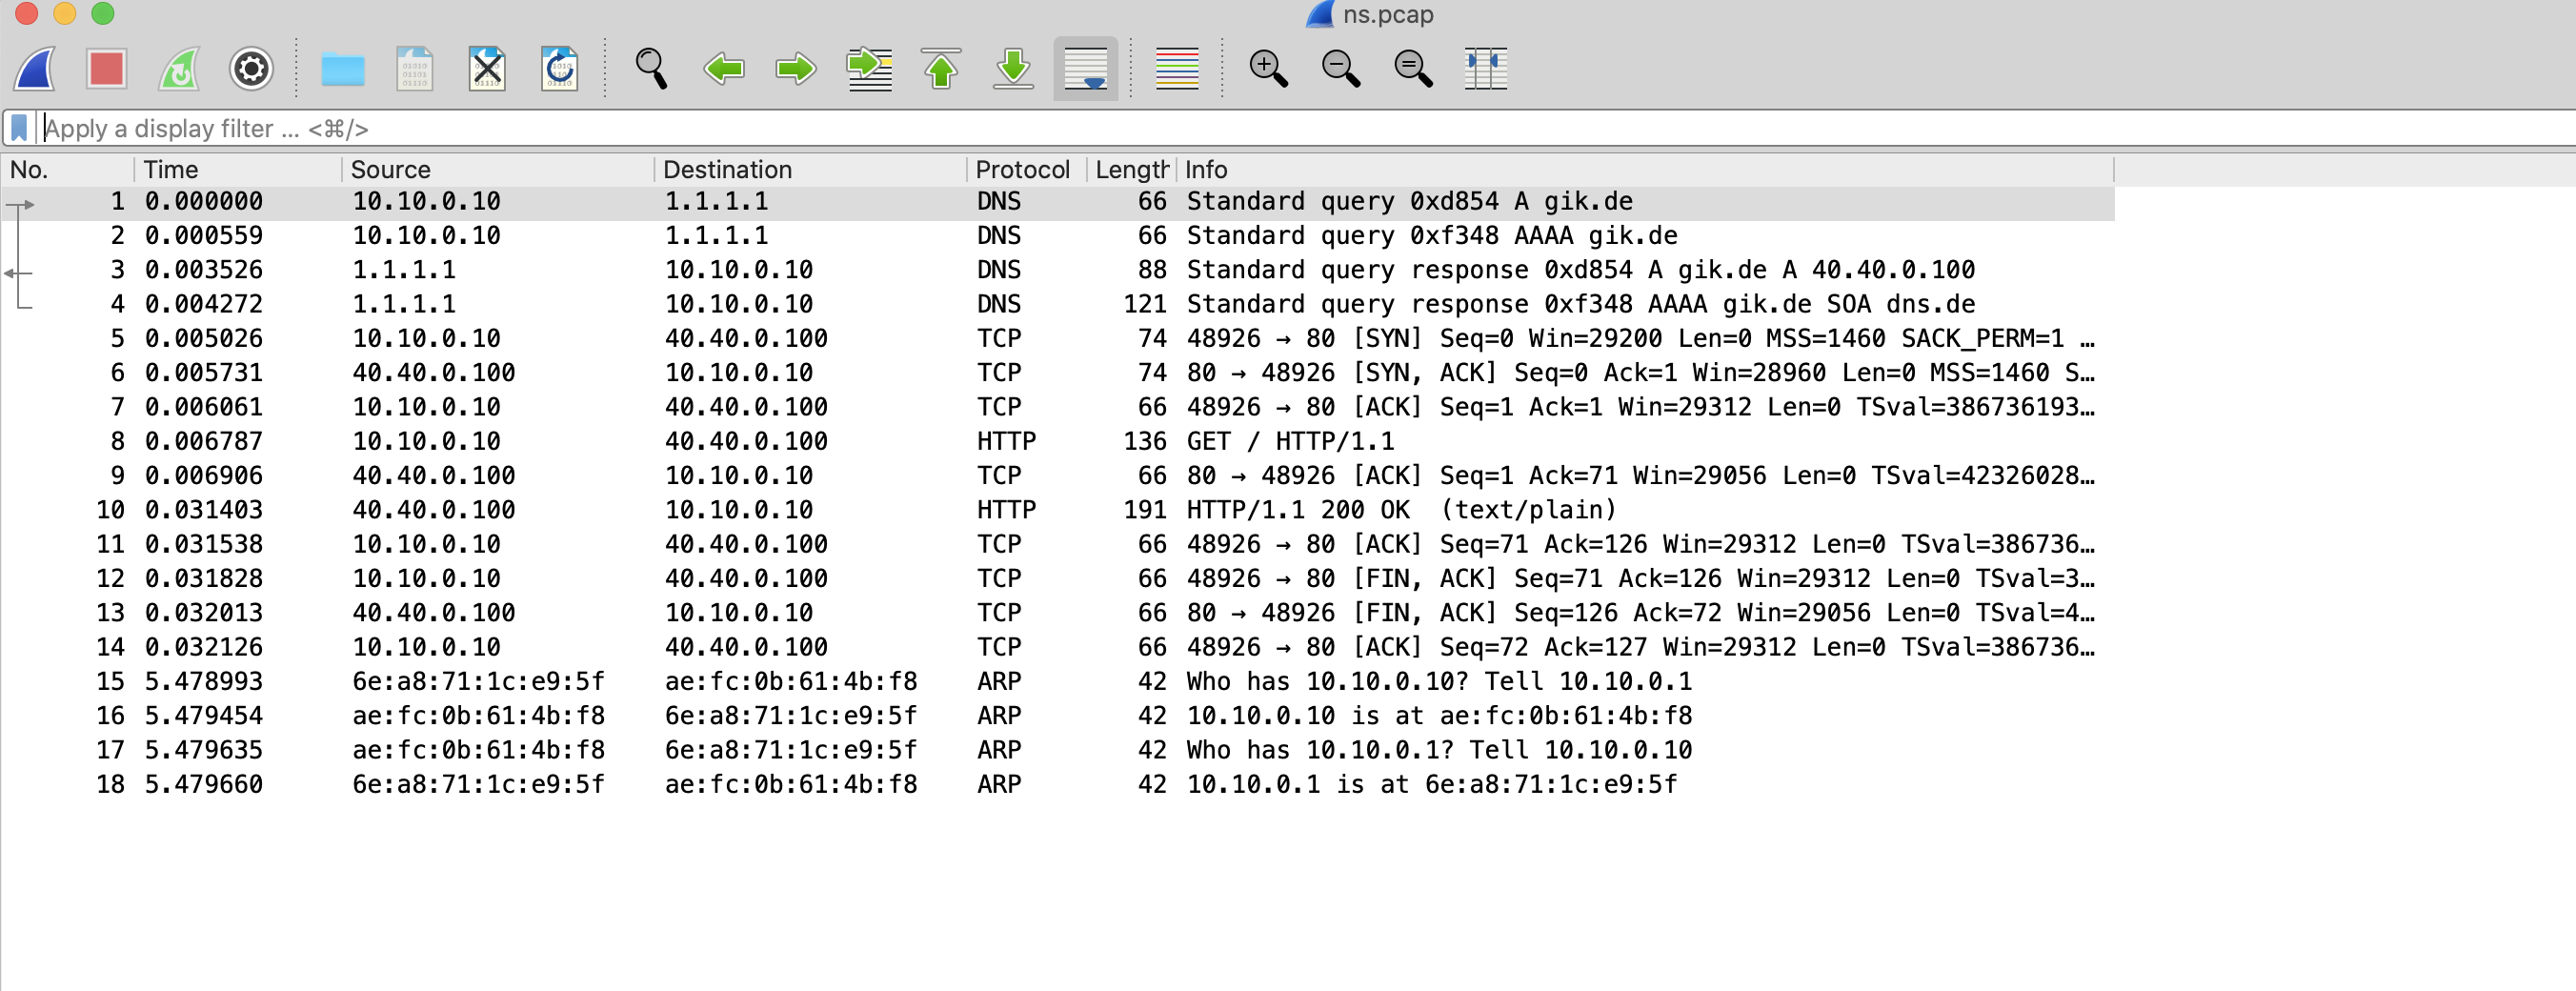
\includegraphics[width=0.9\textwidth]{Images/curlWire.png}
  \caption{Result of Capturing pc1 curl gik.de on wireshark}
  \label{fig:2.7}
\end{figure}

Lets Now explain the steps when you curl gik.de from pc1
\begin{itemize}
\item it begins with pc1 wants to send gik.de a http request so it needs it`s ip address
\item pc1 request for gik.de ip address will be sent to the root domain asking for the ip of gik.de
  \item root domain will reply with where you can find de server and give it web1 ip address
  \item pc1 will send to web1 ip address request asking for the ip of gik.de
  \item web1 will ensure that he can connect with gik.de and will give pc1 the ip of gik.de 
  \item so pc1 now can send directly gik.de http request using gik.de ip address

\end{itemize}

\section{Dig root domain in our case dns\_root}
\begin{figure}[H]
\centering
  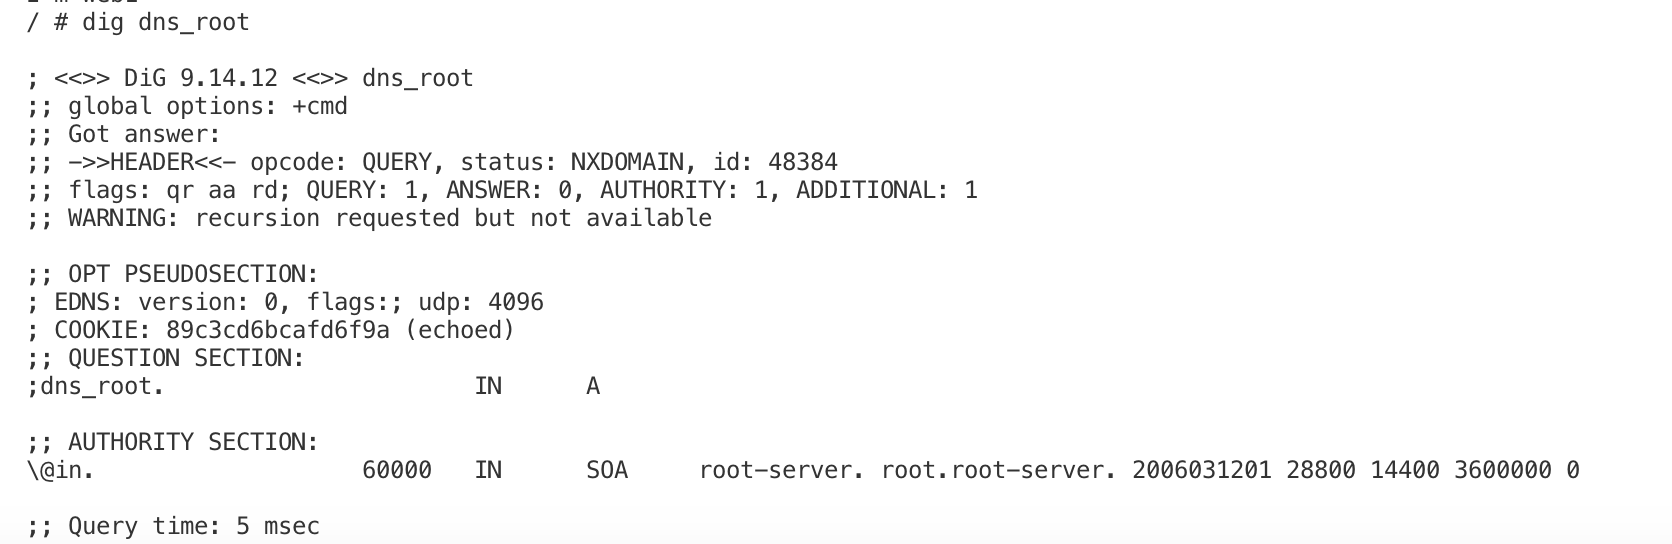
\includegraphics[width=0.9\textwidth]{Images/DigRootDomain.png}
  \caption{Dig root domain}
  \label{fig:2.8}
\end{figure}

\section{DNS server setup at node DNS\_lb }
We will setup dns\_lb to be an authoritative server for the org domain.
The Setup includes creating a folder dns\_lb which contains 2 files.
\subsection{Corefile}
In Corefile of dns\_lb we define 2 server blocks one for each domains we want to route to.The first server block is forwarded to dns\_root where we have setup root domain.
 \begin{figure}[H]
\centering
  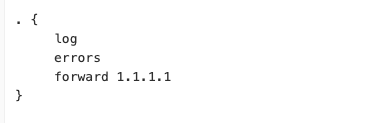
\includegraphics[width=0.9\textwidth]{Images/corefile dns_lb part1.png}
  \caption{Corefile for dns\_root node with server block forwarded to dns\_root}
  \label{fig:2.9}
\end{figure}
\subsubsection{Define Corefile in dns\_lb.startup file}
 \begin{figure}[H]
\centering
  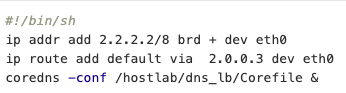
\includegraphics[width=0.9\textwidth]{Images/Corefile declaration in dns_lb.png}
  \caption{Corefile declaration in dns\_lb.startup file}
  \label{fig:2.10}
\end{figure}
\subsection{db.gik.org}
The is DNS zone file, and it will have gik.org name entry.The gik.org points to webservers web bernadette,web amy, and web penny which can we seen in last 3 lines of the file(IP Address).
 \begin{figure}[H]
\centering
  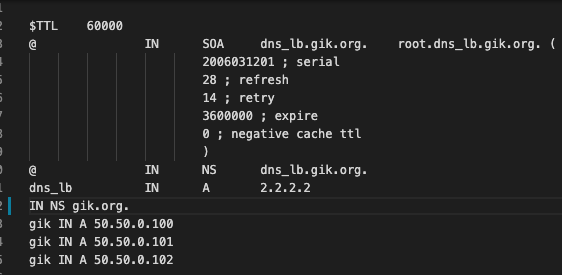
\includegraphics[width=1.2\textwidth]{Images/db.gik.org.png}
  \caption{db.gik.org File }
  \label{fig:2.11}
\end{figure}
\section{Modifying dns\_root to forward name resolution of org to dns\_lb}
In this section we modify the Corefile of dns\_root to forward the gik.org to dns\_lb. 
\begin{figure}[H]
\centering
  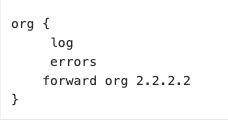
\includegraphics[width=0.9\textwidth]{Images/Forward gik.org to dns_lb.png}
  \caption{Corefile File }
  \label{fig:2.12}
\end{figure}
\section{configure CoreDNS on dns\_lb to load balance the entry gik.org}
DNS load balancing is used to send the DNS requests of the domain to different server machines in order to reduce the load and make the responses faster as there will less load on each of the server machines.
\subsection{Corefile with org server block which handles load balancing}
In this section we add Load balance command:"loadbalance round robin" in corfile within org server block
\begin{figure}[H]
\centering
  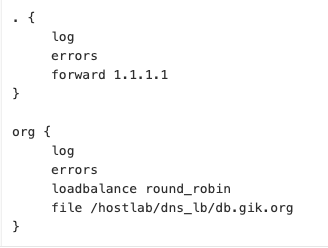
\includegraphics[width=0.9\textwidth]{Images/Load_balance at dns_lb.png}
  \caption{Load Balance at dns\_lb }
  \label{fig:2.13}
\end{figure}
\subsection{Curl gik.org}
we use curl gik.org command to know which server the domain is pointing to.
When we run curl gik.org several times we observe that the domain request is forwarded to same server many times and in random order.
\begin{figure}[H]
\centering
  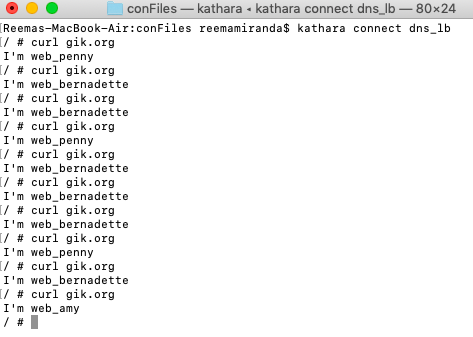
\includegraphics[width=1.2\textwidth]{Images/curl gik.org.png}
  \caption{Curl gik.org execution}
  \label{fig:2.14}
\end{figure}
\subsection{Disadvantages of DNS Load Balancing}
Client request is forwarded to same server destination even if it is overloaded.
We can observe random distribution of request to the servers which leads to traffic congestion.
\section{Dig tool}
\begin{figure}[H]
\centering
  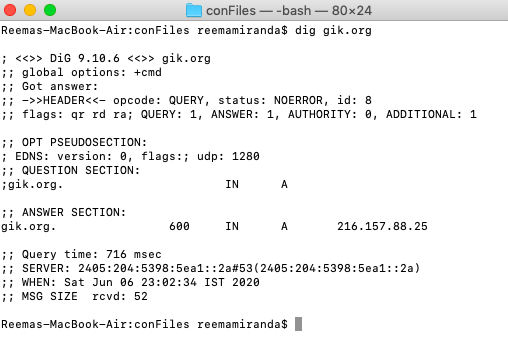
\includegraphics[width=1.3\textwidth]{Images/Dig.png}
  \caption{Dig gik.org execution}
  \label{fig:2.15}
\end{figure}



 